\documentclass[12pt,AutoFakeBold]{article}%第二个参数解决宋体没有粗体的问题
\usepackage{booktabs}%绘制三线表
\usepackage{fontspec}%控制字体
\usepackage[version=3]{mhchem}%化学反应式
\usepackage{xeCJK}%控制中文字体
\usepackage{latexsym}%绘制特殊数学符号
\usepackage[a4paper]{geometry}%纸张大小和页边距
\usepackage{pdfpages}%插入pdf页面
\usepackage{titlesec}%控制标题格
\usepackage{graphicx, epstopdf}%此处使.eps文件可转化成.pdf并应用自动编号功能
\usepackage[journal=angew]{chemstyle}%此处设置图式的样式
\usepackage{siunitx}%数学模式中使用SI单位
\usepackage{color}%提供颜色支持
\usepackage{listings,xcolor}
\usepackage{amsfonts}

\geometry{left=2.5cm,right=2.5cm,top=2.5cm,bottom=2.5cm}%页边距设置
\setmainfont{Times New Roman}%英文字体
\setCJKmainfont{SimSun}%中文字体
\newfontfamily\arial{Arial}%Arial字体
\XeTeXlinebreaklocale "zh"%中文自动换行
\XeTeXlinebreakskip = 0pt plus 1pt%中文自动换行

\newcommand{\dif}{\mathrm{d}}

\begin{document}
    % cover

    % main body
    \section{问题分析}

    \section{模型设计与计算}
    \subsection{模型的基本假设}
    我们的目标是解出高压油管内部压力$p$与时间$t$的关系,这个关系包括一个参数$T$,描述力单向阀每次开启的时长。记作
    \begin{equation}
        p=p(t)
    \end{equation}
    \par
    由条件可见,高压油管的内部体$V$不变,由$\rho=\frac{m}{V}$可见,对高压油管内燃油密度造成影响的仅有高压油管内的燃油质量,用微分方程来表达就是
    \begin{equation}
        \dif\rho=\dif\left(\frac{m}{V}\right)=\frac{\dif m}{V}
        \label{eq1}
    \end{equation}
    \par
    首先我们考虑$\dif\rho$和$p$的关系。\par
    根据注1给出的条件,燃油的压力与其密度具有正相关关系,其关系可以用微分方程
    \begin{equation}
         \begin{cases}
            &\dif p=\frac{E}{\rho}\dif\rho\\
            &p_0=\SI{100}{\MPa},\rho_0=\SI{0.850}{\mg\per\cubic\mm}\\
            &E=E(p)
        \end{cases}
    \end{equation}
    描述,其中$E(p)$由附件3的数据给出,对附件3的数据用MATLAB作图并拟合得到方程,如图\ref{data3}
    \begin{equation}
        E(p)=0.0001p^3-0.001082p^2+5.474p+1532\ \ \ \ (r^2=1.0000)
    \end{equation}
    \begin{figure}[H]
        \centering
        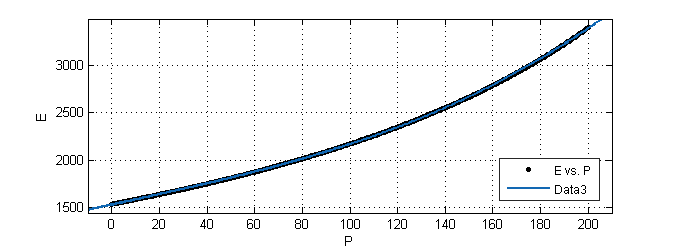
\includegraphics[scale=0.8]{figure/data3.png}
        \caption{燃油弹性模量$E$与压力$p$的非线性拟合结果}
        \label{data3}
    \end{figure}
    由以上的方程我们可以解出关系
    \begin{equation}
        \rho(p)=0.850e^{\int^p_{100}\frac{\dif p}{E(p)}}
        \label{eq2}
    \end{equation}
    \par
    其次,我们再来考虑$\dif m$和$p$与$t$的关系。\par
    $\dif m$由进入和喷出两部分组成。喷出部分对$\dif m$的贡献是时间的函数。单位时间喷出的油量(体积)用函数$Q_{out}(t)$表示,它的解析式在各个小题中有所不同,并且分段可微,所以喷出端造成的$\dif m$可以表述成
    \begin{equation}
        \dif m_{out}=-\rho Q_{out}(t)\dif t
        \label{eq3}
    \end{equation}\par
    进入部分对$\dif m$的贡献也是时间的函数。这个函数含有参数$T$,在上面提及过,它描述了单向阀的开启时间。单位时间进入的油量(体积)用函数$Q_{in}(t)$表示,它的解析式在各个小题中也有所不同,并且分段可微,所以喷出端造成的$\dif m$可以表述成
    \begin{equation}
        \dif m_{in}=\rho Q_{in}(t)\dif t
        \label{eq4}
    \end{equation}\par
    综上,联立方程\ref{eq1}、\ref{eq2}、\ref{eq3}、\ref{eq4},我们可以列出方程
    \begin{equation}
        \frac{\dif p}{E\dif t}=\frac{Q_{in}-Q_{out}}{V}
        \label{maineq}
    \end{equation}\par
    方程\ref{maineq}就是我们对本题建立的基本数学模型。接下来的部分中,我们将根据$Q_{in}(t)$和$Q_{out}(t)$的具体形式,对整个体系最佳$T$值的选择进行讨论。
    
    \subsection{问题1}
    在问题1中$Q_{in}(t)$的形式比较简单,我们定义函数$A=A(t)$来描述供油处入口的截面积,它的形式为
    \begin{equation}
        A(t)=
        \begin{cases}
            \left(\frac{1.4}{2}\right)^2\pi \si{\square\mm} & k(T+10)\leq t\leq k(T+10)+T,k\in\mathbb{N}\\
            0 & k(T+10)+T\leq t\leq (k+1)(T+10),k\in\mathbb{N}
        \end{cases}
    \end{equation}
    代入题目中给出的流量公式可得
    \begin{equation}
        Q_{in}(t)=CA(t)\sqrt{\frac{2(p_{high}-p)}{\rho}}
    \end{equation}\par
    在问题1中$Q_{out}(t)$的形式也比较简单,它是由题目中图\ref{inputof1}给出的
    \begin{figure}[H]
        \centering
        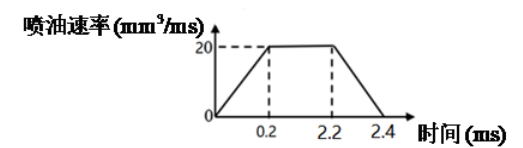
\includegraphics[scale=0.75]{figure/inputof1.png}
        \caption{问题1中的喷油速率}
        \label{inputof1}
    \end{figure}
    写成函数为
    \begin{equation}
        Q_{out}(t)=
        \begin{cases}
            100t&100k\leq t\leq 100k+0.2,k\in\mathbb{N}\\
            20&100k+0.2\leq t\leq 100k+2.2,k\in\mathbb{N}\\
            -100t+240&100k+2.2\leq t\leq 100k+2.4,k\in\mathbb{N}\\
        \end{cases}
    \end{equation}\par
    将$Q_{in}(t)$和$Q_{out}(t)$的具体形式代入方程\ref{maineq},发现所得方程是一阶常微分方程,所以尝试用差分法通过计算机进行数值解微分方程,取$\Delta t=\SI{0.01}{ms}$,用Wolfram Mathematica计算并绘制出对应于不同$T$取值$p-t$变化图\ref{ptfigure1}
    \begin{equation}
        \frac{p_{i+1}-p_i}{E(p_i)\Delta t}=\frac{1}{V_0}\left(CA(ti)\sqrt{\frac{2\left(p_h-p_i\right)}{\rho_h}}-Q_{out}(t_i)\right)
    \end{equation}
    \begin{figure}[H]
        \centering
        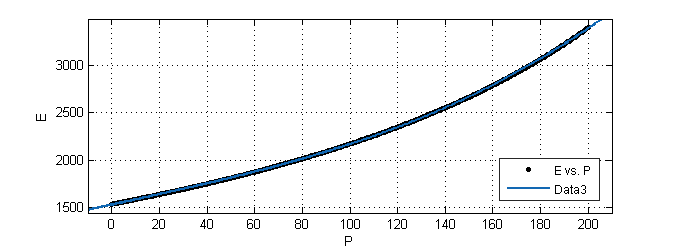
\includegraphics[scale=0.8]{figure/data3.png}%notnow!
        \caption{差分方程数值模拟结果}
        \label{ptfigure1}
    \end{figure}
    利用二分法C++程序可以解出精确到百分位的$T$值$T=$
    % appendix
        
\end{document}